\subsection{Reconstruction and Identification}
\par When a $\tau$ lepton decays hadronically it is referred to 
as a hadronic $\tau$, otherwise it is reconstructed as the electron or muon that 
it decays to (See Sections~\ref{sec:ele} and \ref{sec:mu}). In either case, there is a $\nu_\tau$
in the final decay products. Since this $\nu_\tau$ is invisible in the ATLAS detector the hadronic $\tau$ 
is reconstructed through its visible decay products, which are referred to as $\tauvis$.
As discussed in Section~\ref{sec:sm} the $\tau$ lepton is restricted to decaying to an 
odd number of charged mesons, with decreasing branching ratios as the odd number increases. 
In ATLAS the most common hadronic $\tau$ decays constitute 1 or 3 charged pions, sometimes with associated 
neutral pions. 

\subsubsection{Reconstruction}
\par The $\tauvis$ signature in ATLAS comprises some energy deposits in the 
calorimeters, matched to 1 or 3 ID tracks.\footnote{$\geq$5 ID tracks are very rare.} 
$\tauvis$ with 1 matched track are 
called {\it 1-prong}, and those with 3 matched tracks are called {\it 3-prong}. 
Since neutral pions decay as $\pizero\to\gamma\gamma$, a significant component of the energy is deposited in 
the electromagnetic calorimeters for those $\tau$ lepton decays that include neutral pions. 

\par The largest background to the hadronic $\tau$ 
is the QCD jet, although electrons and muons can be reconstructed as $\tauvis$ as well. 
With a smaller transverse mass, $\tauvis$ components from a hadronic $\tau$ tend to be more 
collimated than those from a QCD jet for a given $\pt$. Moreover, due to higher particle 
multiplicity in a QCD jet, a QCD jet tends to have a higher ID track multiplicity  
than a hadronic $\tau$ for a given $\pt$. These two differences are used to reduce the QCD jet 
background contamination, as discussed in Section~\ref{sec:idTauJets}.
     
\par Topological clusters in all jets with $\pt>10~\GeV$ and $|\eta|<2.5$, reconstructed as discussed in Section~\ref{sec:jets},
 are used as seeds by the $\tau$ reconstruction algorithm. Tracks from the ID that satisfy a 
the selection criteria shown in Table~\ref{tab:tautrkSel} are matched to the $\tauvis$ candidate,  
using the center of the vector sum of all the topological 
clusters (henceforth known as the $\tauvis$ center) as reference. This reference point 
may not be the same as the center of the reconstructed jet 
because the jet center undergoes corrections described in Section~\ref{sec:jetCalib}.
Tracks from the ID that lie within $\Delta R<0.2$ around the $\tauvis$ center are counted 
as tracks from the $\tau$ decay. The $\tau$ candidate is then classified as either 1-prong 
or 3-prong, depending on the number of tracks found within $\Delta R<0.2$. 
Energy from topological clusters that lie within $\Delta R<0.2$ around the $\tauvis$ center are summed up to compute the 
total transverse energy $\eT$ of the $\tauvis$ candidate, which is taken as equal to $\pT$, on account 
of the small $\tau$ lepton mass. The 
$\tauvis$ is then characterized by $\pt,\eta$ and $\phi$, where $\eta,\phi$ are 
the $\tauvis$ center coordinates. 
Further, the following regions in relation to the $\tauvis$ center are defined:

\begin{enumerate}
\item $\Delta R<0.1$, as the {\it calo-core} region;
\item $\Delta R<0.2$, as the {\it core} region;
\item and $0.2<\Delta R<0.4$, as the {\it isolation ring}.
\end{enumerate} 

\begin{table}[!h]
\centering
   \begin{tabular}{|c|}
\hline
{\bf Selection Criteria} \\
\hline\hline \\
$\pt>1~\GeV$ \\
Number of b-Layer hits $\geq 1$ \\
Number of Pixel Detector hits $\geq 2$ \\
Number of Silicon Detector hits $\geq 7$ \\
$|d_0|<1.0$ mm \\
$|z_0\sin\theta|< 1.5$ mm \\ 
\hline
   \end{tabular}
\caption{Selection criteria for tracks from the Inner Detector that are matched to $\tau$-jet candidates.}
\label{tab:tautrkSel}
\end{table}

\subsubsection{Identification against QCD Jets}
\label{sec:idTauJets}
\par To further reduce the fraction of QCD jets that are reconstructed as $\tauvis$, a separate 
identification algorithm is applied on the reconstructed hadronic $\tau$ lepton. Several variables,
 designed to exploit the differences in shower width and track multiplicity between 
hadronic $\tau$ jets and QCD jets, are used. Only a few are discussed here, but for a more detailed discussion the reader should 
consult Ref~\cite{ATLAS:tauvars}. 

\begin{enumerate}
\item 
\begin{equation*}
f_{\text{core}} = \frac{\sum_{i\in\text{calo-core}} E_{T,i}^{EM}}{ \sum_{j}^{\Delta R_i\in\text{core}} E_{T,j}^{EM}}
\end{equation*}
is the fraction of transverse energy deposited in topological clusters in the core-calo region, to that deposited in the core
 region. The energy deposits are calibrated at the EM scale. For studies used in this analysis, 
a more pile-up robust version of this variable is $f_{\text{core}}^{\text{corr}}$ used, 
after correcting for pile-up events by taking into account the number of vertices with at least 2 tracks in the event.  

\item 
\begin{equation*}
f_{\text{track}} = \frac{\pT^{\text{leadTrk}}}{ \sum_{j\in\text{core}} E_{T,j}^{EM}}
\end{equation*}
is the ratio of the transverse momentum of the track with the highest transverse momentum, to energy deposits in the core 
region of the $\tauvis$. Here, a pile-up corrected version $f_{\text{track}}^{\text{corr}}$ is used, just like in the 
$f_{\text{core}}$ case. 

\item 
\begin{equation*}
R_{\text{track}} = \frac{\sum_i^{\Delta R_i<0.4}(\pti\times\Delta R_i)}{\sum_i^{\Delta R_i<0.4} \pti} 
\end{equation*}
is the transverse radius defined by the $\tauvis$ tracks, weighted by the \pt\ of the tracks. 

%\item 
%\begin{equation*}
%R_{had} = \frac{\sum_{i\in\{Had\}}^{\Delta R_i<0.4} (E_{T,i}\times\Delta R_i)}{ \sum_{i\in\{Had\}}^{\Delta R_i<0.4} E_{T,i}}
%\end{equation*}
% is  
%defined as the $\tauvis$ transverse radius in the hadronic component of the calorimeter. It is a ratio of the 
%distance-weighted sum of hadronic topoclusters energies to their unweighted sum. The expectation is that $\tau$ leptons would 
%generally have a smaller $R_{had}$ than QCD jets.  
%
%\item 
%\begin{equation*}
%R_{cal} = \frac{\sum_{i\in\{EM\}}^{\Delta R_i<0.4} (E_{T,i}\times\Delta R_i)  + \sum_{i\in\{Had\}}^{\Delta R_i<0.4} (E_{T,i}\times\Delta R_i) }{ \sum_{i\in\{EM\}}^{\Delta R_i<0.4} E_{T,i} + \sum_{i\in\{Had\}}^{\Delta R_i<0.4} E_{T,i} }
%\end{equation*}
% is defined 
%as the $\tauvis$ transverse radius in all calorimeter components. 
%It is similar to $R_{had}$, differing in that it includes topoclusters from the electromagnetic calorimeters. 
%$R_{cal}$'s expectations are similar to those of $R_{had}$.
%
\end{enumerate}

\par Some variables were showed stronger discrimination strength when applied either to 1-prong 
or 3-prong $\tauvis$. For example, for 1-prong $\tauvis$ candidates the impact parameter 
significance ($d_0/\delta d_0)$ of the track  with the highest \pT, and the number of tracks in the 
isolation ring are used. For 3-prong $\tauvis$ candidates the maximal $\Delta R$ between the $\tauvis$
tracks and its center, and the invariant mass of the track system are used. 

\par With these and other variables each $\tauvis$ candidate lies in a multivariate hyper-space. Monte-Carlo 
simulations are used to train Boosted Decision Trees (BDTs).
\Ztautau\ and \Wtaunu\ events from simulated samples are used as signal to train the 
BDT on $\tau$ leptons while QCD multi-jets from data are used to train the BDT on QCD jets. 
The BDT is trained in several distinct categories to maximize its classification 
strength. The first categorization is $n$-prong, separating the candidates according to their 
associated tracks.
The second categorization is the reconstructed $\tau$ \pt. The \pt\ ranges are 
0$\to$45~\GeV, 45$\to$100~\GeV, and 100$\to\infty$~\GeV. The last categorization is the number of 
vertices in the event, to get a handle on pileup effects. The number of vertices are 
categorized into ranges of 1$\to$3, 4$\to$7, and 8$\to\infty$.   

\par There are three working points for $\tau$ identification. {\it Loose} is defined at a target signal 
selection efficiency of 70\% for 1-prong and 65\% for 3-prong $\tauvis$. Likewise, the {\it medium} 
working point targets a signal efficiency of 60\% for 1-prong and 55\% for 3-prong $\tauvis$. Lastly, 
the {\it tight} working point targets a signal efficiency of 40\% for 1-prong and 35\% for 3-prong.  
%Figure~\ref{fig:tauEff} shows identification efficiencies of signal and background as a function of 
%$\pt$ and the number of vertices, categorized into the number of prongs. 
%
%\begin{figure}[h]
%%   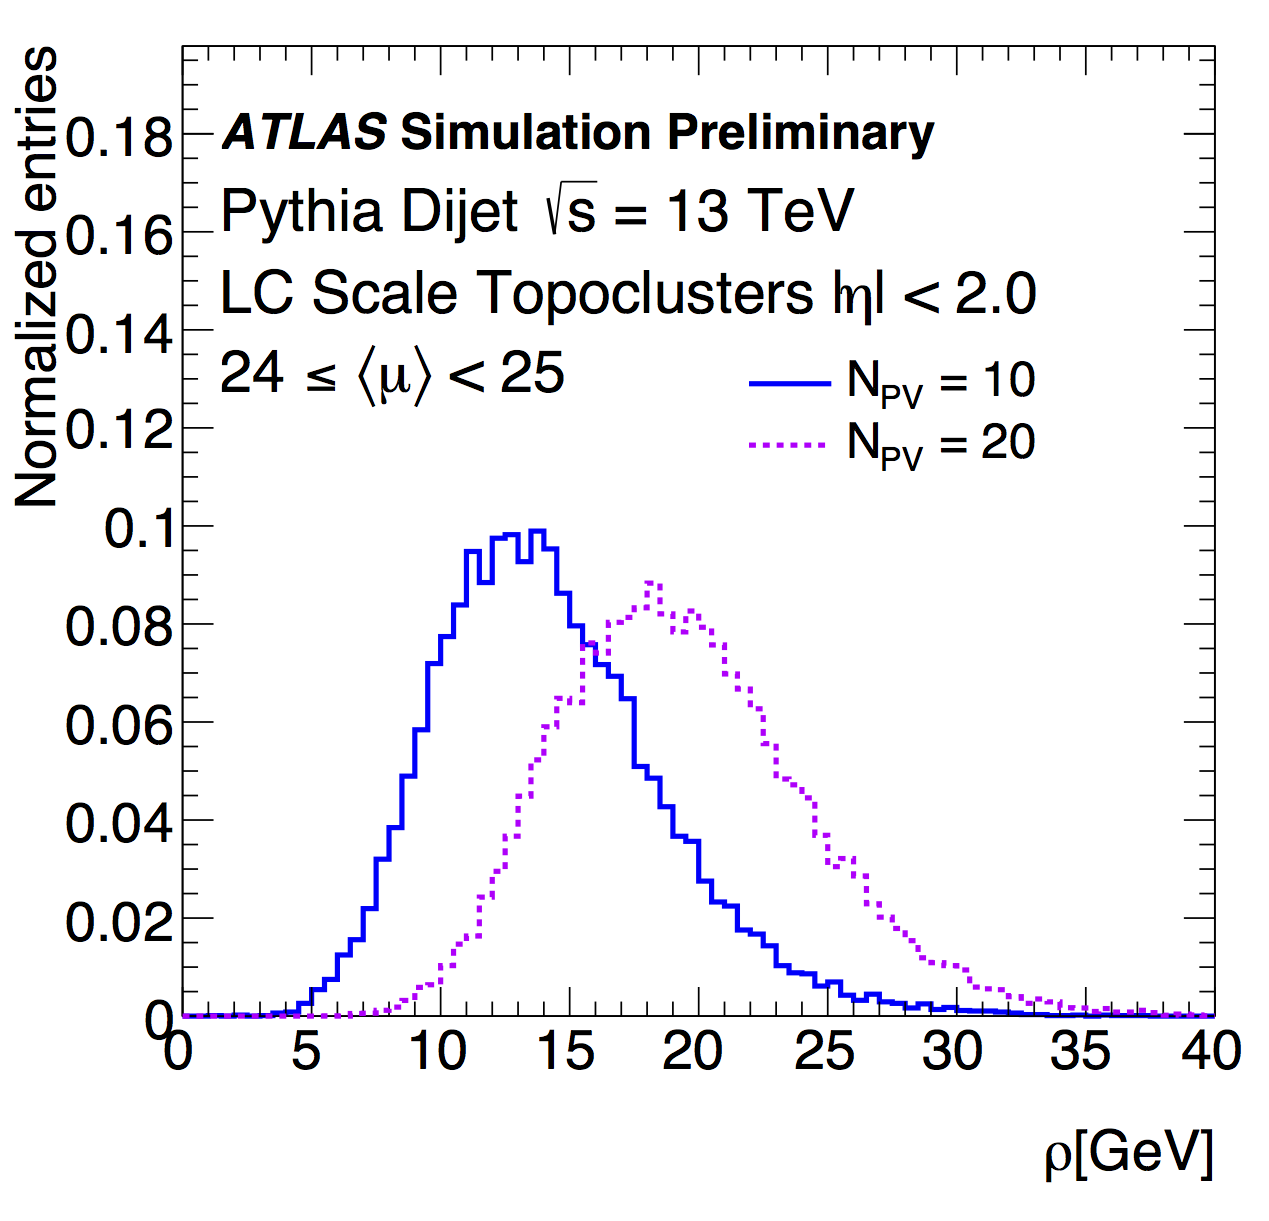
\includegraphics[width=\textwidth]{figures/rho13.png}
%\rectangle{\linewidth}{0.5cm}
%	\caption{Identification efficiency distributions for hadronic $\tau$ leptons and for QCD jets (background)} 
%	\label{fig:tauEff}
%\end{figure}

\subsubsection{Identification against electrons and muons}
\par As already hinted, electrons and muons may also be reconstructed as hadronic $\tau$ leptons. 
This is more common for electrons than it is for muons because muons rarely deposit most of their 
energy in the calorimeters. Since an electron is likely to be associated with one track, 1-prong 
$\tauvis$ suffer a lot more electron contamination than 3-prong electrons. 

\par A BDT is used to train hadronic $\tau$ signal and electron backgrounds. Monte Carlo simulation samples of 
$\Ztautau$ and $\Zee$ are used for these respective tasks. Both the electron and $\tau$ candidates 
are required to pass $\pT>20~\GeV$. The $\tauvis$ is further required to pass the BDT loose 
selection criteria. Upon overlap between and electron and a $\tauvis$, an electron is preferred.    
The BDT was trained in categories of $|\eta|<1.37, 1.37<|\eta|<2.0, 2.0<|\eta|<2.3$ and 
$|\eta|>2.3$.

\par Apart from $f_{\text{core}}^{\text{corr}}, f_{\text{track}}^{\text{corr}}$ and $R_{\text{track}}$
 some variables that enhanced electron/$\tau$ separation were used. These are 
\begin{enumerate}
\item 
\begin{equation*}
f_{iso} = \frac{\sum_{i\in\text{isolation ring}}E_{T,i}^{EM}}{\sum_{j}^{\Delta R<0.4} E_{T,j}^{EM}},
\end{equation*}
compares the width of the electron and $\tauvis$ showers. Although the electron shower is not expected 
to be much wider than the $\tauvis$ shower, some differences at the core level are expected;

\item and $f_{\text{HT}}$, the ratio of high-threshold to low-threshold hits in the TRT. Electrons, being 
lighter than pions (from the $\tau$ decay), have higher Lorentz factors ($\gamma$). So they are 
expected to produce more high-threshold hits in the TRT than hadronic $\tau$ leptons.  
\end{enumerate} 

%\par Figure~\ref{fig:eleTauEff} shows identification efficiencies of signal and background, 
%categorized in $\eta$. 
%
%\begin{figure}[h]
%%   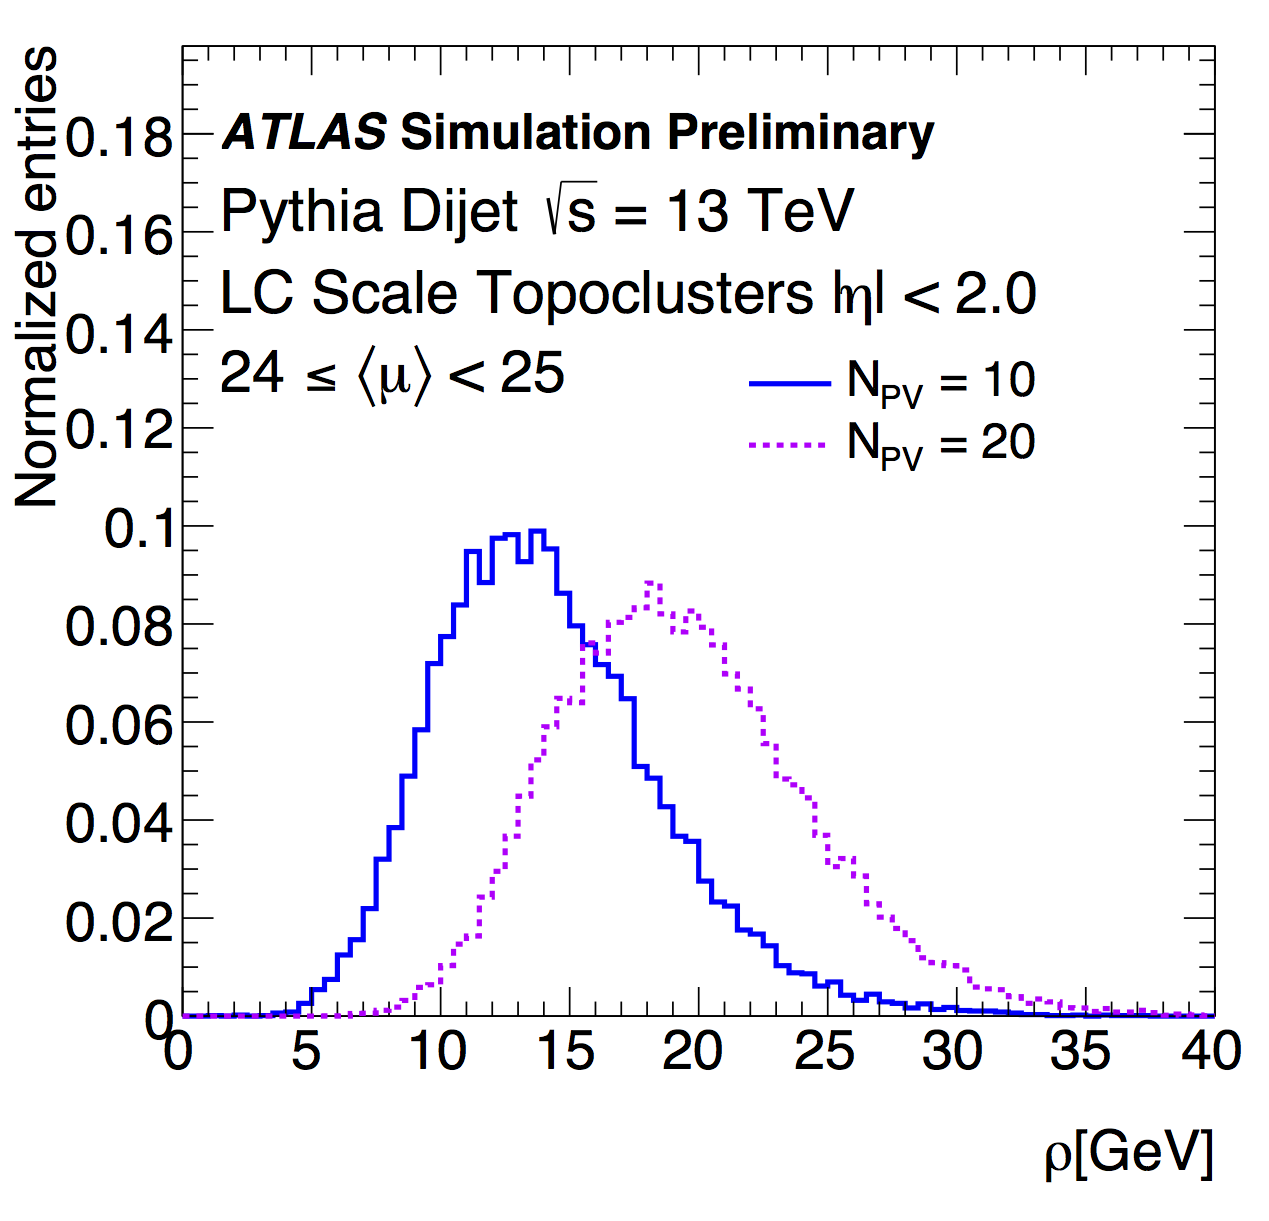
\includegraphics[width=\textwidth]{figures/rho13.png}
%\rectangle{\linewidth}{0.5cm}
%	\caption{Identification efficiency distributions for hadronic $\tau$ leptons and for electrons (background)} 
%	\label{fig:eleTauEff}
%\end{figure}
%
%\par Muons ...
%****
%muons
%****
% 1. only two variables used ... fTrack and fEM
% 2. In my code no scale factors seem to be applied though ... Confused.
%
%\subsubsection{Identification Efficiency}
%TO DO ... Describe in detail how identification efficiencies for MC are extracted and applied
% 1. objective is to calculate eff in data, and in sim and obtain scale factors
% 2. eff in sim is trivial because the tauvis is matched to truth
% 3. eff in data is obtained in a dedicated region
% 4. this region in practice has backgrounds. they need to be quantified
% 5. choose a variable that's good at separating background and signal (extended Ntracks)
% 6. get predictions of variable for expected signal, background and fit to data
% 7. perform fit before and after ID, as they change

% 1. Ztautau events
% 2. Wtau
% 3. ttbar 


%\subsection{Systematic Uncertainties}
